\section{Experimentación}

Hicimos unas pruebas del tiempo de ejecución de las dos versiones de

\begin{center}
	\texttt{static pair<string, uint> ConcurrentHashMap::maximum\\(uint p\_archivos, uint p\_maximos, list<string> archs);}
\end{center}

correspondientes a los ejercicios 5 y 6 del trabajo práctico. La versión del ejercicio 5 no utiliza la versión concurrente de \texttt{ConcurrentHashMap::count\_words}, y la versión del ejercicio 6 (llamada \texttt{maximum\_6} para desambiguar) sí.

\begin{center}
	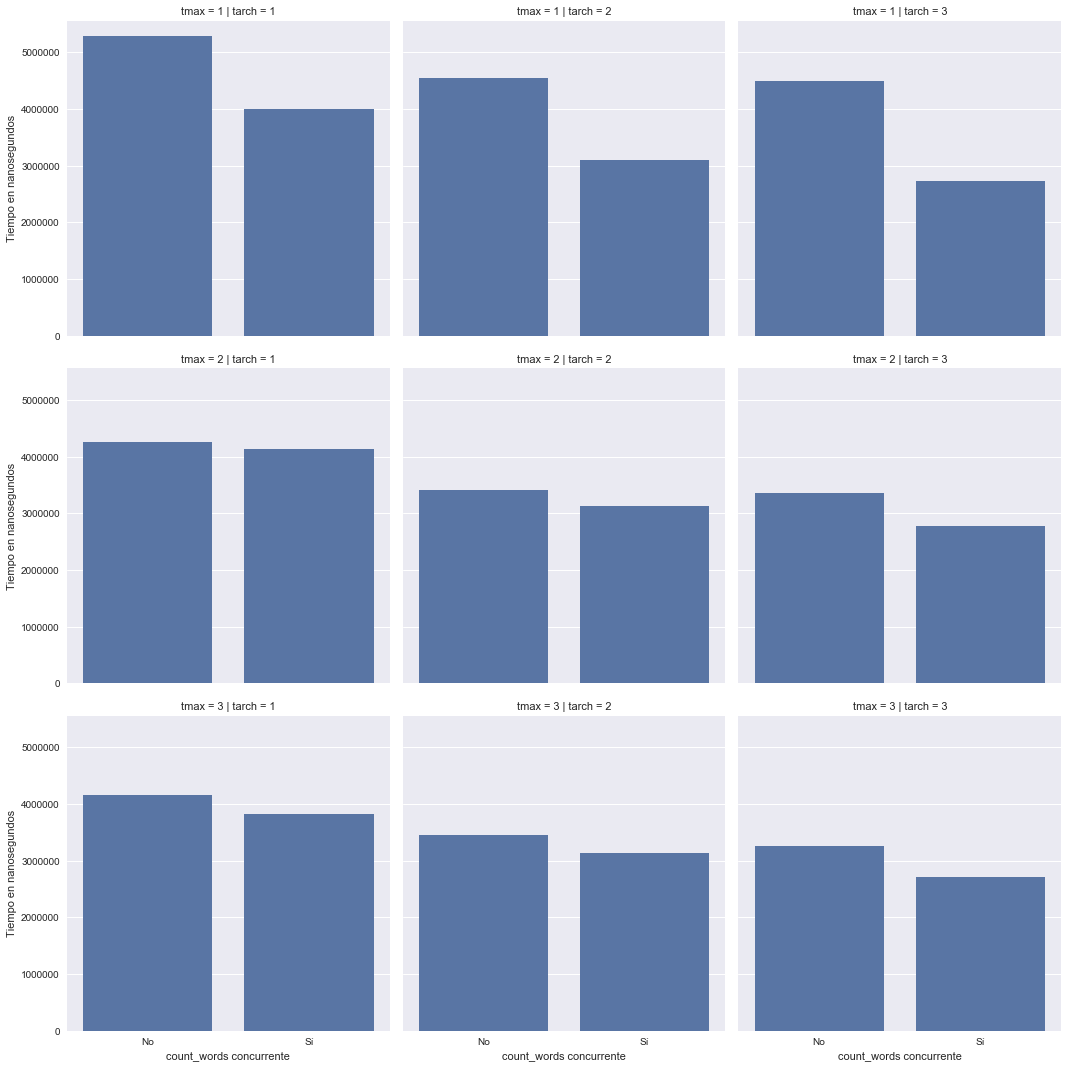
\includegraphics[scale=0.45]{imgs/5-vs-6.png}
\end{center}

En este gráfico se pueden apreciar 2 cosas:

\begin{itemize}

	\item la mejora de performance al utilizar threads es muy notoria, aunque la diferencia al agregar el 2do thread es mayor a la de agregar el 3er thread;

	\item la función que utiliza la versión con concurrencia de \texttt{ConcurrentHashMap::count\_words} puede hacer mejor uso de los threads que tiene disponibles, en particular durante la carga de los archivos, lo que era esperable ya que en la versión no concurrente se generan varios HashMaps y se deben copiar esos resultados a un único HashMap. También suponemos que, dado que todos los HashMaps almacenan sus datos en orden y tienen mutexes por fila de la tabla, es posible que haya muchas esperas durante la copia al HashMap unificado.

\end{itemize}